\section{Implementation}\label{sec:implementation}

\begin{figure}[H]
\centering
\begin{minted}{python}
def satisfiable(p: Proposition, backend_or_sampler, is_backend: bool) -> bool:
    oracle, atom_lookup = phase_oracle(p)
    grover_op = grover(oracle, atom_lookup)
    N = 2 ** count_atomic_propositions(p)
    m = 1
    while m <= math.sqrt(N):
        k = random.randint(1, round(m))
        grover_k_times = QuantumCircuit(grover_op.num_qubits)
        grover_k_times.h(list(range(len(atom_lookup))) + [grover_op.num_qubits - 1])
        for _ in range(k):
            grover_k_times.compose(grover_op, inplace=True)
        grover_k_times.measure_all()
        if is_backend :
            grover_k_times = transpile(grover_k_times, backend_or_sampler)
            result = (
                backend_or_sampler.run(grover_k_times, shots=1).result().get_counts()
            )
        else:
            result = backend_or_sampler.run([grover_k_times], shots=1).result()[0].data.meas.get_counts()
        result_bit_string = next(iter(result))[::-1]
        witness_assignment = {}
        for atom in atomic_propositions(p):
            witness_assignment[atom] = char_to_bool(
                result_bit_string[atom_lookup[atom]]
            )
        if valuation(p, witness_assignment):
            return True
        m = (5 / 4) * m
    return False
\end{minted}
\caption{Implementation of \mintinline{python}{satisfiable} }
\label{fig:satisfiable}
\end{figure}

\subsection{\texttt{phase\_oracle} Implementation}

\autoref{fig:oracle} should give an idea of the circuit that \texttt{phase\_oracle} returns, however, there are some differences: The circuit produced by \texttt{phase\_oracle} only has one output bit, and the result is encoded in the phase instead of the bit.
This is done because the \texttt{GroverOperator} function, provided by Qiskit, expected such a circuit.

\begin{figure}[H]
    \centering
    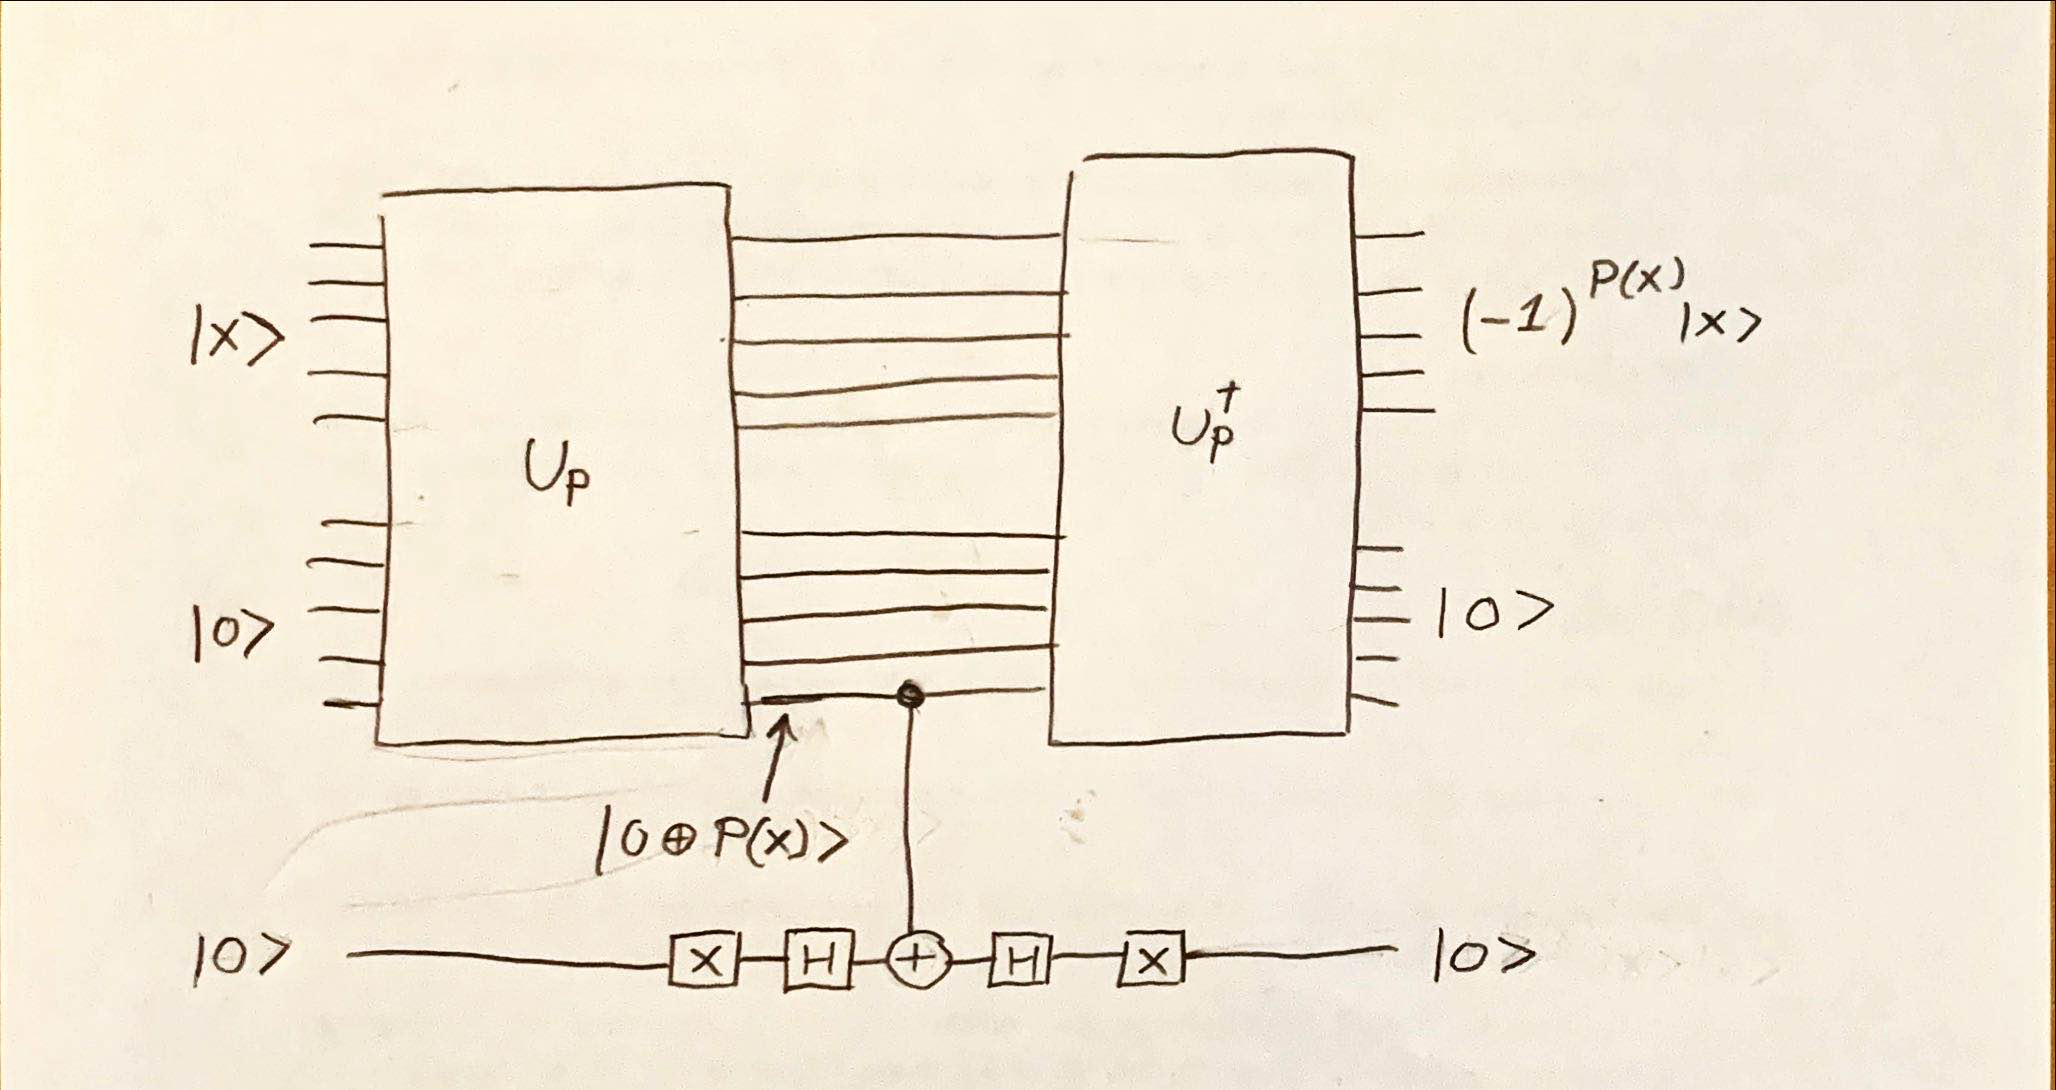
\includegraphics[width=\textwidth]{figures/garbage-free-computation.jpg}
    \caption{Oracle circuit}
    \label{fig:oracle}
\end{figure}

First off, on line 1, a lookup table relating atomic propositions to their location inside the circuit is created.
This lookup table is returned along with the circuit.
Further, in line 2, the base circuit where qubits corresponding to atomic propositions reside is created.
On line 3, the circuit $R$ is created, this is further described in \autoref{subsubsec:phase-oracle-recur-implementation}.
On line 6 through 12 the result is encoded in the phase of a separate qubit, by sandwiching a controlled not gate, depending on the result of $R$, between a not and Hadamard gate.
Finally, on line 13 through 15, $R^\dagger$ is created and added to the circuit, and the circuit and lookup table are returned.

\begin{figure}[H]
\centering
\begin{minted}{python}
def phase_oracle(p: Proposition) -> Tuple[QuantumCircuit, Dict[str, int]]:
    atom_lookup = {item: index for index, item in enumerate(atomic_propositions(p))}
    qc_base = QuantumCircuit(len(atom_lookup))
    qc_r = phase_oracle_recur(p, qc_base, atom_lookup)
    qc_r_r_daggert_pos = list(range(0, qc_r.num_qubits))
    qc_final = QuantumCircuit(qc_r.num_qubits + 1)
    qc_final.compose(qc_r, qc_r_r_daggert_pos, inplace=True)
    qc_final.x(qc_final.num_qubits - 1)
    qc_final.h(qc_final.num_qubits - 1)
    qc_final.cx(qc_final.num_qubits - 2, qc_final.num_qubits - 1)
    qc_final.h(qc_final.num_qubits - 1)
    qc_final.x(qc_final.num_qubits - 1)
    qc_r_daggert = qc_r.inverse()
    qc_final.compose(qc_r_daggert, qc_r_r_daggert_pos, inplace=True)
    return qc_final, atom_lookup
\end{minted}
\caption{Implementation of \mintinline{python}{phase_oracle} }
\label{fig:phase_oracle}
\end{figure}

\subsubsection{\texttt{phase\_oracle\_recur} Implementation}\label{subsubsec:phase-oracle-recur-implementation}

The implementation of \texttt{phase\_oracle\_recur} and thus the construction of $R$ proceeds by recursion on the structure of the proposition \texttt{p}.

The base case, when \texttt{p} is an atomic proposition, is handled on line 4 through 8.
In this case the location of the qubit corresponding to the atomic proposition is found, and a fanout is created introducing a new qubit, as shown in \autoref{fig:fanout}.
Note that only basis states are copied, as general copying of quantum states is impossible.

\begin{figure}[H]
    \centering
    
\includegraphics[width=\textwidth]{figures/FANOUT-with-CNOT.jpg}
    \caption{FANOUT gate}
    \label{fig:fanout}
\end{figure}

The first recursive case, when \texttt{p} is the negation of some proposition \texttt{p.not\_p}, is handled on line 9 through 12.
In this case we recurse on \texttt{p.not\_p} and add a NOT gate to the result qubit of the resulting circuit.

The second recursive case, when \texttt{p} is two propositions \texttt{p.p1}, \texttt{p.p2} connected by some connectivity (either $\land$ or $\lor$), is handled on line 13 through 34.
In this case we recurse on the two propositions \texttt{p.p1}, \texttt{p.p2} and the resulting circuits are combined in the following manner:
First the part of the circuit where the atomic propositions reside, ignoring fanouts, are combined at the top of the circuit.
Then the rest of the resulting circuits are stacked upon each other.
Finally, a result bit is added at the bottom as indicated by \autoref{fig:and-not-gates}.
In figure \autoref{fig:and-not-gates} the location of the top two qubits correspond the location of the result qubits in the resulting circuits of \texttt{p.p1} and \texttt{p.p2}.

\begin{figure}[H]
    \centering
    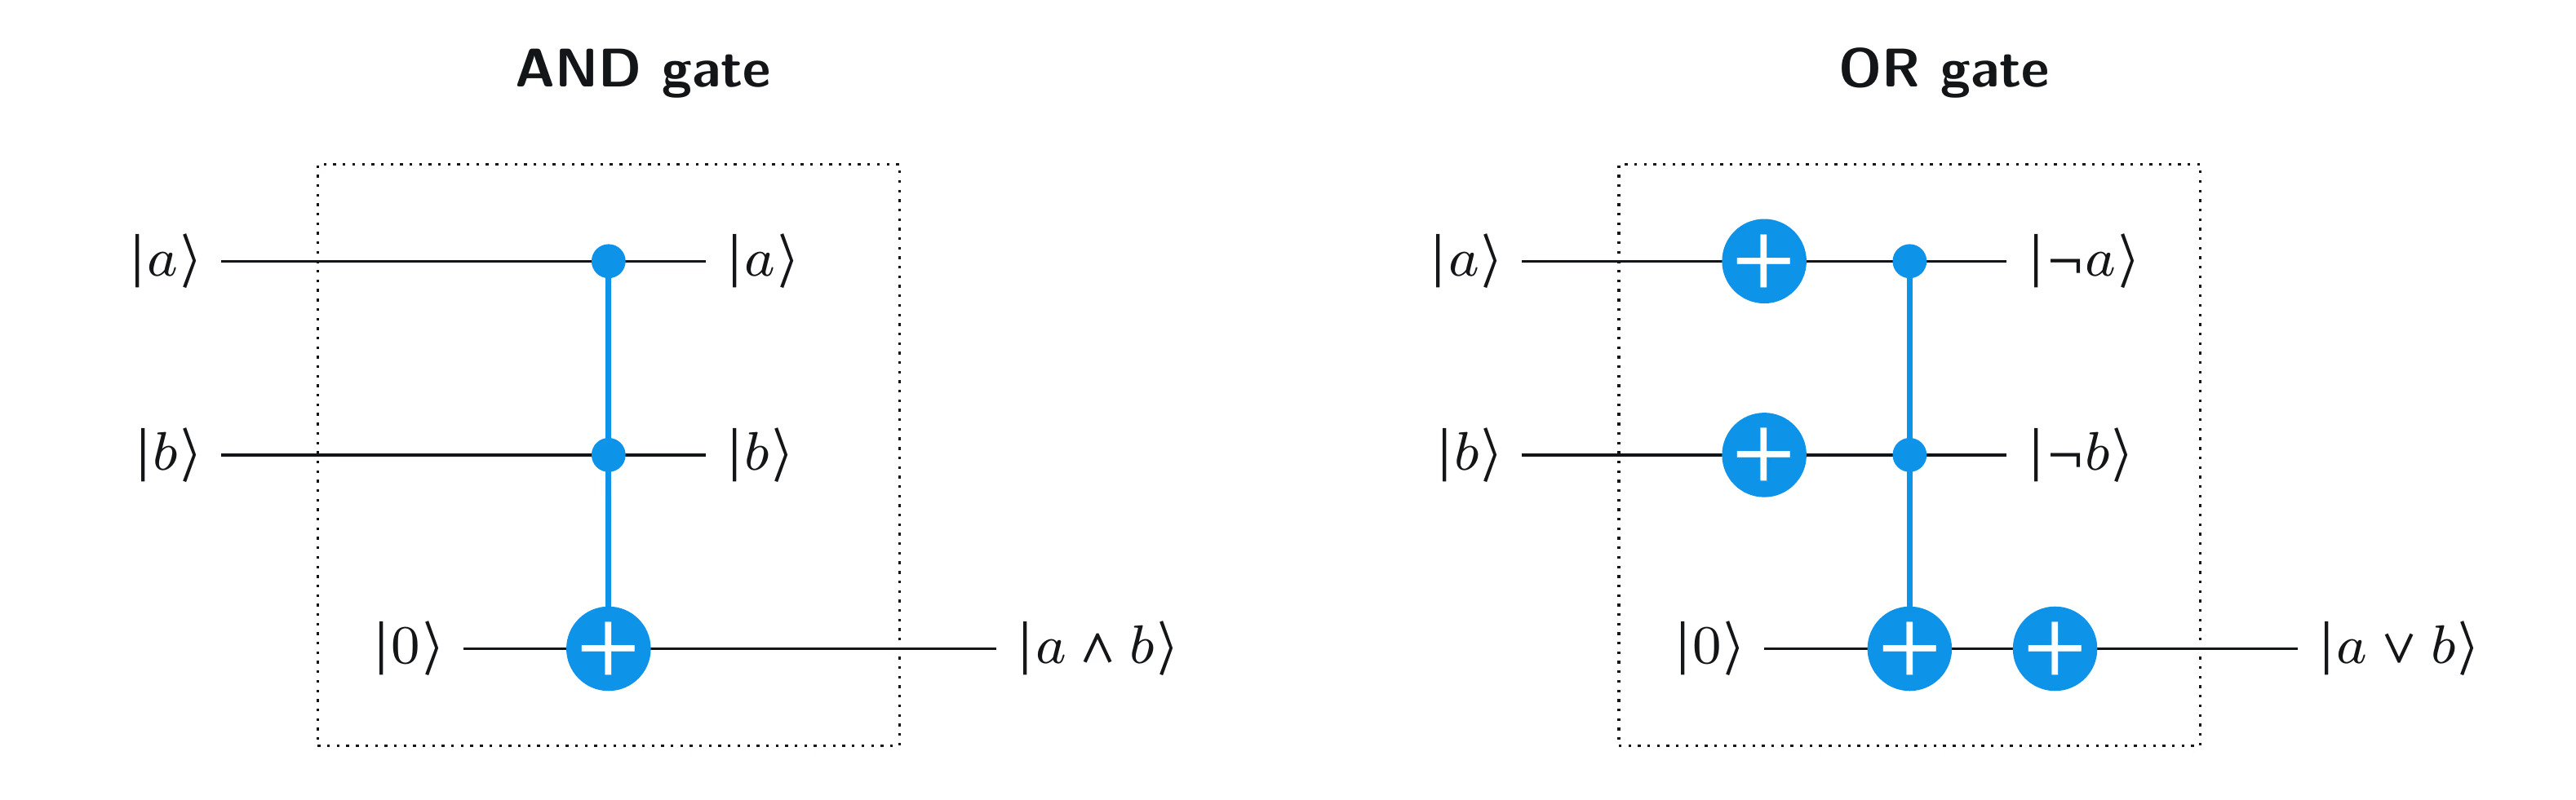
\includegraphics[width=\textwidth]{figures/AND-and-OR-with-Toffoli.jpg}
    \caption{AND and NOT gates}
    \label{fig:and-not-gates}
\end{figure}

\begin{figure}[H]
\centering
\begin{minted}{python}
def phase_oracle_recur(
    p: Proposition, qc_base: QuantumCircuit, atom_lookup: Dict[str, int]
) -> QuantumCircuit:
    if type(p) is Atomic:
        qc_atom = QuantumCircuit(qc_base.num_qubits + 1)
        qc_atom.cx(atom_lookup[p.id], qc_base.num_qubits, f"atom {p.id}")
        qc_atom.compose(qc_base, list(range(1, qc_base.num_qubits + 1)))
        return qc_atom
    if type(p) is Negation:
        qc_pnot = phase_oracle_recur(p.not_p, qc_base, atom_lookup)
        qc_pnot.x(qc_pnot.num_qubits - 1)
        return qc_pnot
    if type(p) is Conjunction or Disjunction:
        qc_1 = phase_oracle_recur(p.p1, qc_base, atom_lookup)
        qc_2 = phase_oracle_recur(p.p2, qc_base, atom_lookup)
        qc_base_start = 0
        qc_base_end = qc_base_start + qc_base.num_qubits
        qc_base_range = list(range(qc_base_start, qc_base_end))
        qc_1_start = qc_base_end
        qc_1_end = qc_1_start + qc_1.num_qubits - qc_base.num_qubits
        qc_2_start = qc_1_end
        qc_2_end = qc_2_start + qc_2.num_qubits - qc_base.num_qubits
        qc_junction = QuantumCircuit(qc_2_end + 1)
        qc_1_range = qc_base_range + list(range(qc_1_start, qc_1_end))
        qc_junction.compose(qc_1, qc_1_range, inplace=True)
        qc_2_range = qc_base_range + list(range(qc_2_start, qc_2_end))
        qc_junction.compose(qc_2, qc_2_range, inplace=True)
        if type(p) is Disjunction:
            qc_junction.x(qc_1_end - 1)
            qc_junction.x(qc_2_end - 1)
        qc_junction.ccx(qc_1_end - 1, qc_2_end - 1, qc_junction.num_qubits - 1)
        if type(p) is Disjunction:
            qc_junction.x(qc_junction.num_qubits - 1)
        return qc_junction
\end{minted}
\caption{Implementation of \texttt{phase\_oracle\_recur} }
\label{fig:phase_oracle_recur}
\end{figure}

\subsection{\texttt{grover} Implementation}\label{subsec:grover-implementation}

The code seen in \autoref{fig:grover} is how our implementation handles the construction of the Grover operation on the given proposition p, represented as its corresponding quantum circuit.
In line 2, we construct a quantum circuit which has the same size as the oracle.
This is going to be used for representing which qubits of the oracle we want affected by the Grover operation.

Then in line 3--5, we set up a hadamard gate to be used on the basis state qubits; these being each qubit representing an atom of the proposition and the result qubit.
This is being done on the previously constructed quantum circuit, \texttt{qc\_state\_prep}, essentially ignoring the so-called workspace qubits, and only focusing on the ones in basis state.
The reason for doing this is that we only want to apply the Grover operation to the basis state qubits.

In line 6, we then select and make a list of the same qubits as the prequel.
The reason for this are the parameters needed for the GroverOperator, G, constructor in line 7.
This is a class already defined in Qiskit, which defines a Grover operator representing a single run through the unitary algorithm, namely $G=H^{\bigotimes n}Z_{OR}H^{\bigotimes n}Z_f$ as stated in~\cite{Grover}.
Here, $Z_{OR}$ is being handled by the class, to which we gave the reflection qubits selected in line 7 and the quantum circuit, \texttt{qc\_state\_prep}.

Our oracle is then equivalent to the $Z_f$ operation of the algorithm.

At last, in line 10, we return the constructed Grover operator such that it can be used as a tool in going through the algorithm, as seen in \autoref{fig:oracle}.

\begin{figure}
\centering
\begin{minted}{python}
def grover(oracle: QuantumCircuit , atom_lookup: Dict[str, int]) -> QuantumCircuit:
    qc_state_prep = QuantumCircuit(oracle.num_qubits)
    qc_state_prep.h(oracle.num_qubits - 1)
    for i in range(len(atom_lookup)):
        qc_state_prep.h(i)
    reflection_qubits = list(range(len(atom_lookup))) + [oracle.num_qubits - 1]
    grover_op = GroverOperator(
        oracle, qc_state_prep, reflection_qubits=reflection_qubits
    )
    return grover_op
\end{minted}
\caption{Implementation of \mintinline{python}{grover} }
\label{fig:grover}
\end{figure}


